% Created 2024-05-19 Sun 23:53
% Intended LaTeX compiler: xelatex
\documentclass[a4paper,11pt,twoside]{article}
\usepackage{graphicx}
\usepackage{longtable}
\usepackage{wrapfig}
\usepackage{rotating}
\usepackage[normalem]{ulem}
\usepackage{amsmath}
\usepackage{amssymb}
\usepackage{capt-of}
\usepackage{hyperref}
\usepackage{libertine}
\usepackage[left=3cm, right=3cm, top=3 cm, bottom=3cm]{geometry}
\author{Ryan Lynch}
\date{\today}
\title{Intro. to Unity's Input System}
\hypersetup{
 pdfauthor={Ryan Lynch},
 pdftitle={Intro. to Unity's Input System},
 pdfkeywords={},
 pdfsubject={},
 pdfcreator={Emacs 29.3 (Org mode 9.6.24)}, 
 pdflang={English}}
\usepackage{biblatex}

\begin{document}

\maketitle
\section*{Introduction}
\label{sec:org1d76761}
This walk-through is intended to get you up and running with Unity's event driven \textbf{Input System}. It is a brief summarization that does not get into the details behind it. For that go to \href{https://gamedevbeginner.com/input-in-unity-made-easy-complete-guide-to-the-new-system/}{Input in Unity made easy}, which is also the source that this demo is based on.
In this example we'll create \textbf{Input Actions} for a player. We'll create common actions that a player might create in a game.
\section*{Installing the Input System}
\label{sec:org4f675d4}
In the editors top menu bar, Navigate to \emph{(Window > Package Manager)}
\begin{center}
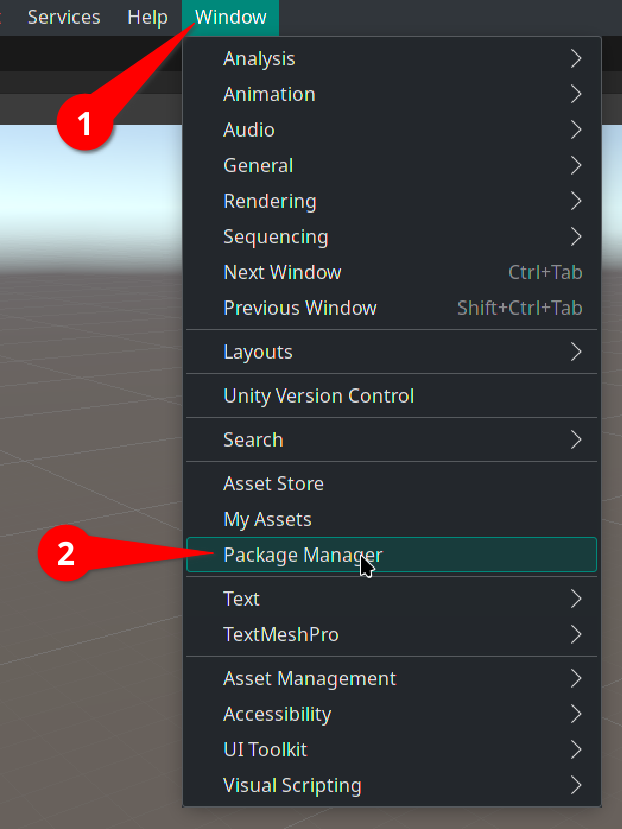
\includegraphics[width=.9\linewidth]{./SnapShots/PackageManager.png}
\end{center}
To install the input system:
\begin{enumerate}
\item Select the \emph{``Unity Registry''}
\item Search for the \emph{``Input System''}
\item Select \emph{``Install''}
\end{enumerate}
\begin{center}
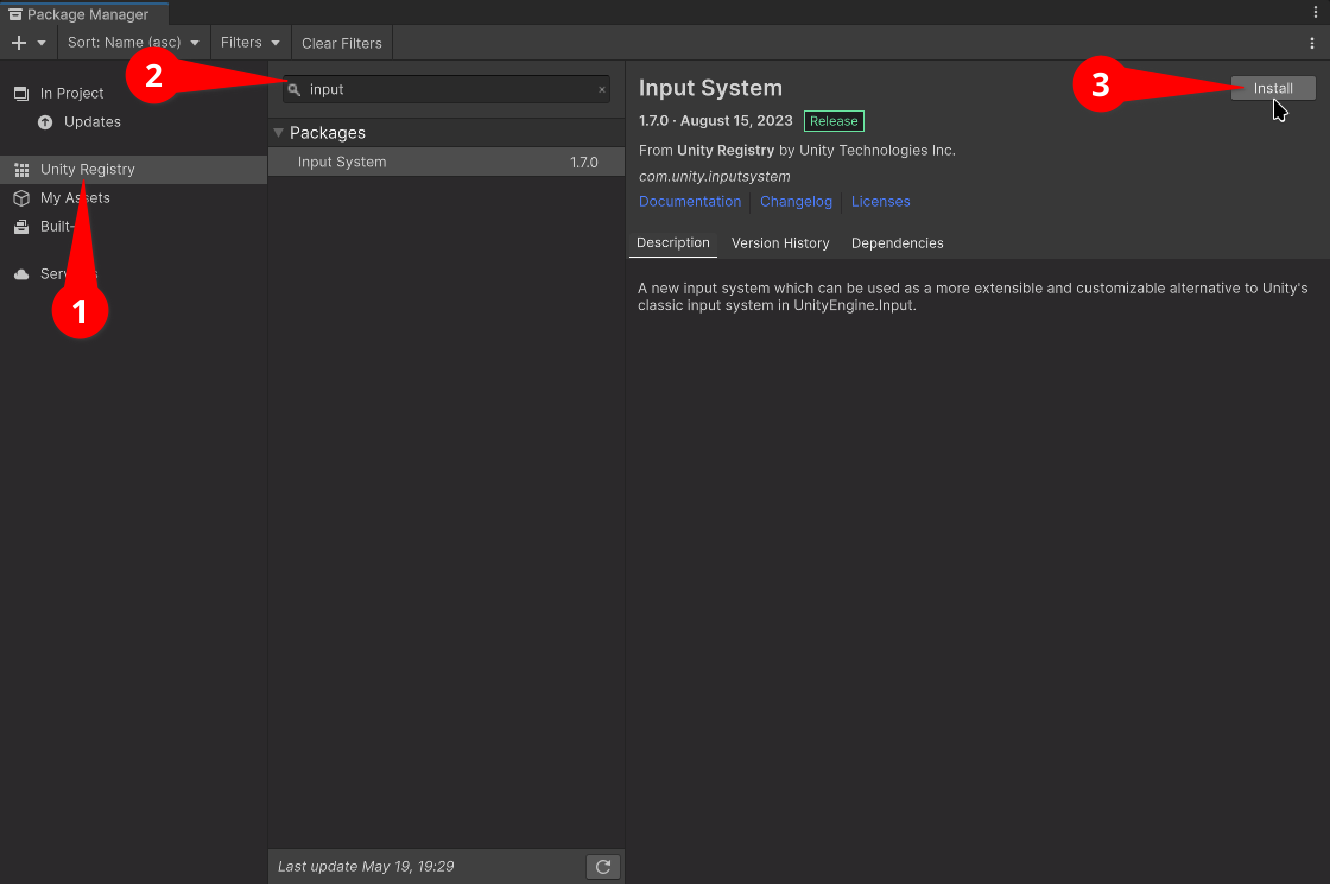
\includegraphics[width=.9\linewidth]{./SnapShots/Installing.png}
\end{center}
Unity will proceed to install the \textbf{Input System} Package. You should now restart your Unity Editor.
\section*{Creating Input Actions}
\label{sec:org03ccaf4}
\textbf{Input Actions} represent events that take place in your game. These events are triggered from some input like a keyboard, mouse or gamepad.
\subsection*{Create a New Input Action Asset}
\label{sec:orgfbad295}
An \textbf{Input Action Asset} represents a collection of \textbf{Action Maps}. This makes working with \textbf{Action Maps} more intuitive from the editor.
In the editors top menu bar, Navigate to \emph{(Assets > Create > Input Actions)}
\begin{center}
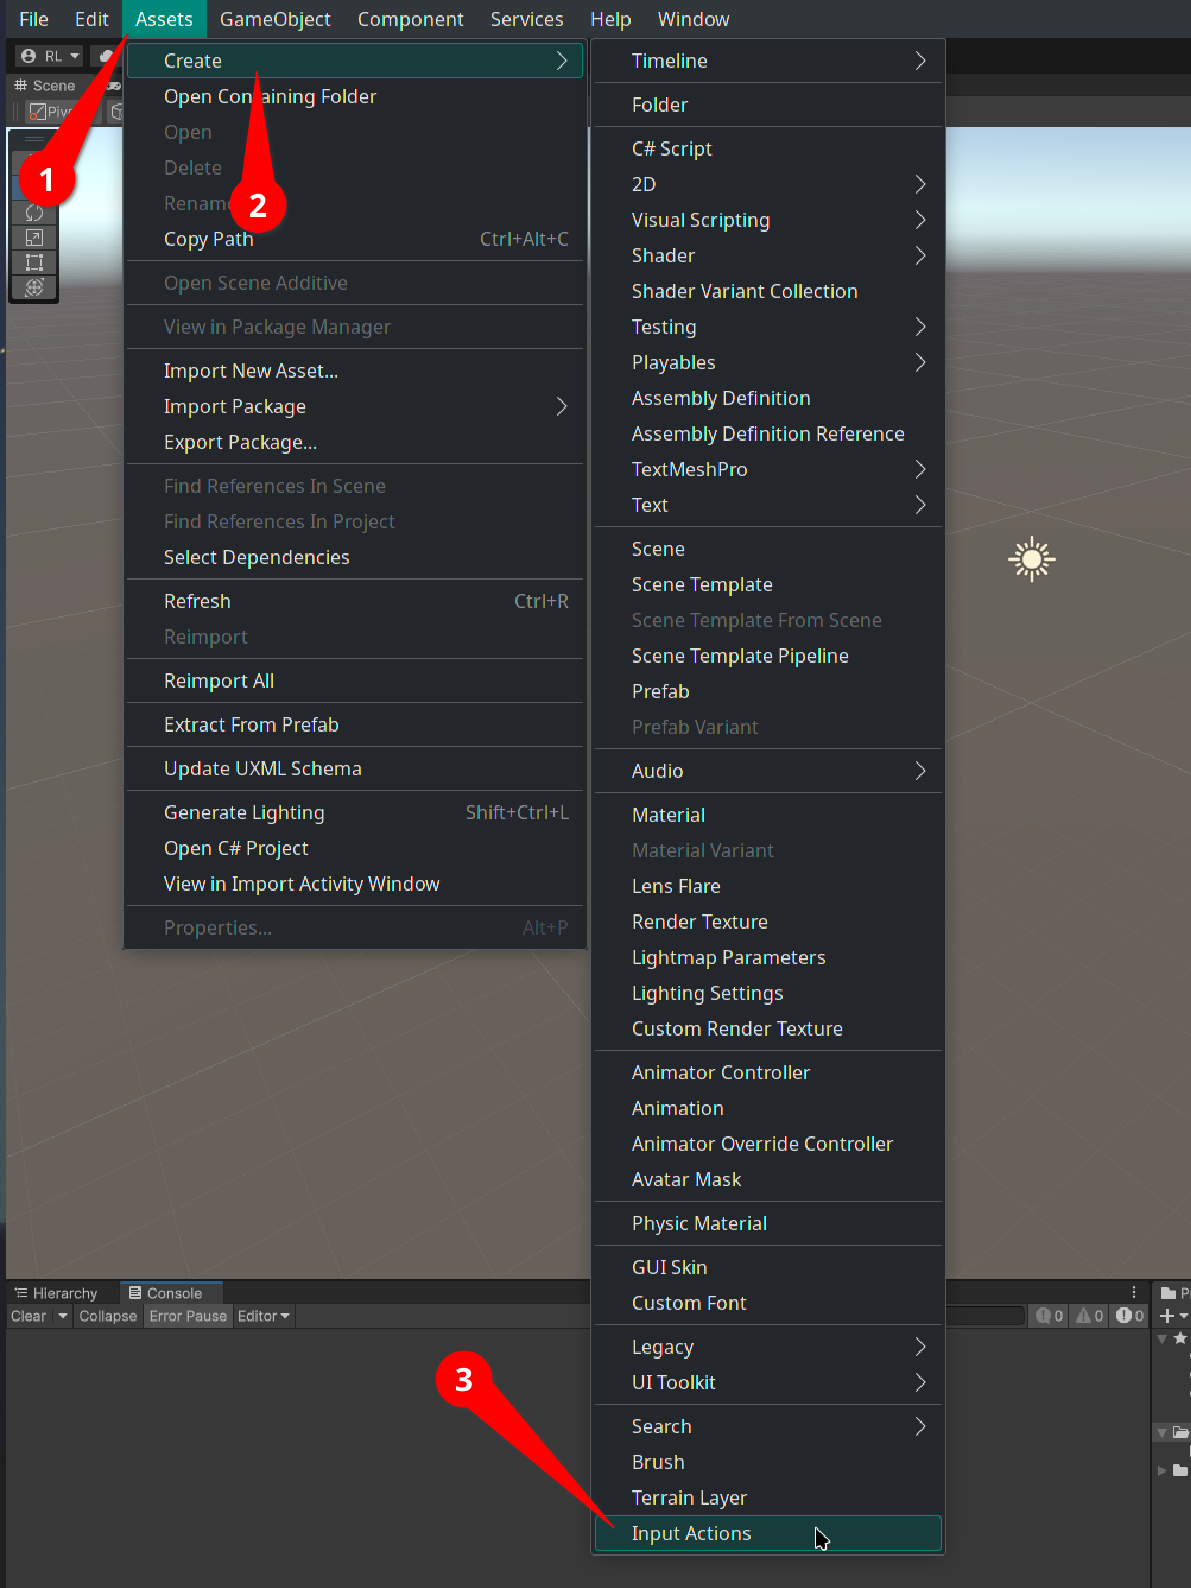
\includegraphics[width=.9\linewidth]{./SnapShots/InputActionAsset.png}
\end{center}
In our example we name this \textbf{Input Action Asset} \emph{``PlayerInputActions''}.
\subsection*{Configure Control Scheme}
\label{sec:orga90cb95}
\textbf{Control Schemes} represent the input devices that will trigger our \textbf{Input Actions}.
Double clicking the \textbf{Input Action Asset} we just created in the editor, opens a new window.
\begin{enumerate}
\item Select the \emph{``No Control Schemes''} drop down menu
\item Select \emph{``Add Control Scheme\ldots{}''}
\end{enumerate}
\begin{center}
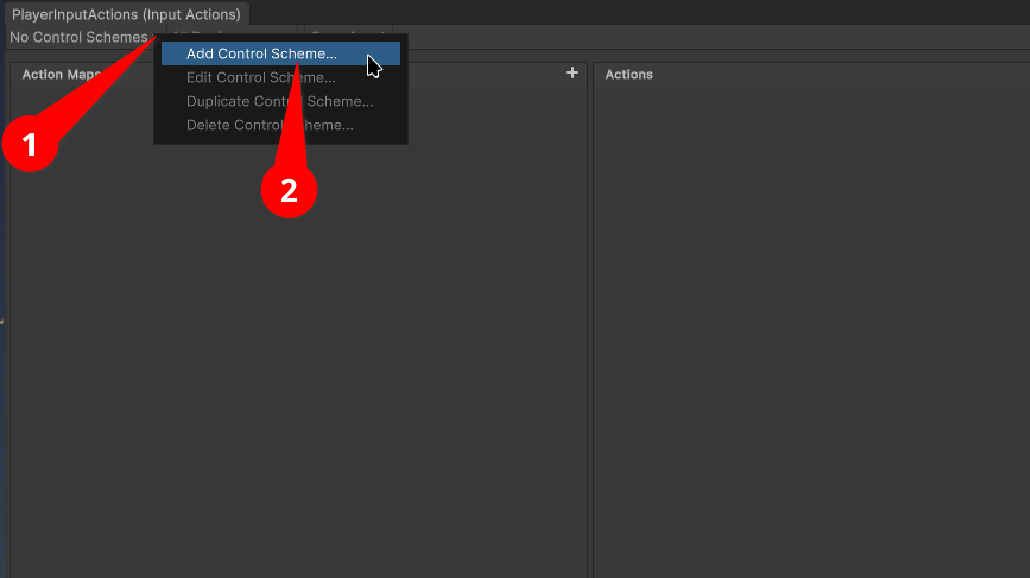
\includegraphics[width=.9\linewidth]{./SnapShots/ControlScheme.png}
\end{center}
In our example we create a new scheme called \emph{``Keyboard\&Mouse''}. We attach the \emph{``[Keyboard]''} and \emph{``[Mouse]''} devices to this scheme.
\begin{enumerate}
\item Click the plus button under the \emph{``List is Empty''} UI.
\item Search for the \emph{``[Keyboard]''} device inn the search bar
\item Select the \emph{``[Keyboard]''} devices in the search results
\item Repeat these steps 1-3 for the \emph{``Mouse''} device
\item Select \emph{``Save''}
\end{enumerate}
\begin{center}
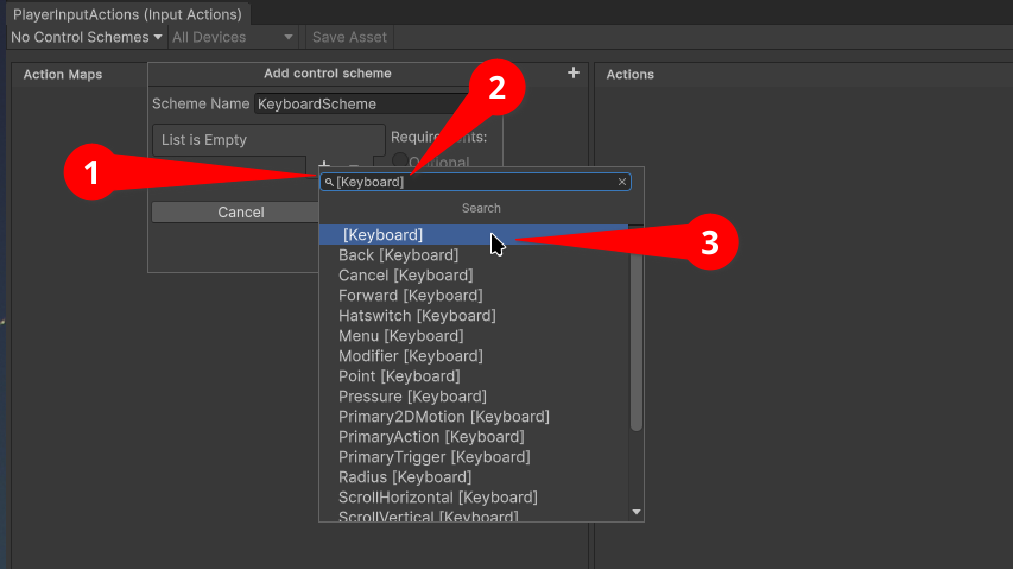
\includegraphics[width=.9\linewidth]{./SnapShots/AddScheme.png}
\end{center}
Our new scheme will be selected automatically because it is our only scheme. Be sure to check the \emph{``Auto-Save''} box to save the changes we make in the \textbf{Input Actions} editor.
\begin{center}
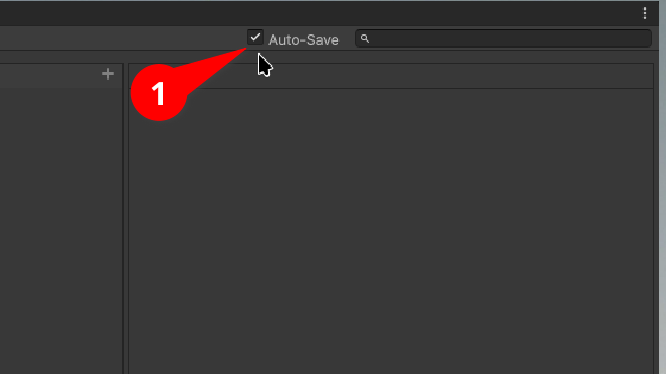
\includegraphics[width=.9\linewidth]{./SnapShots/Auto-Save.png}
\end{center}
\subsection*{Create a New Action Map}
\label{sec:orgb350d20}
We'll create a new \textbf{Action Map} for our player. This holds all the \textbf{Input Actions} related to our player.
\begin{enumerate}
\item Select the \emph{``+''} icon in the \emph{``Action Maps''} panel
\end{enumerate}
\begin{center}
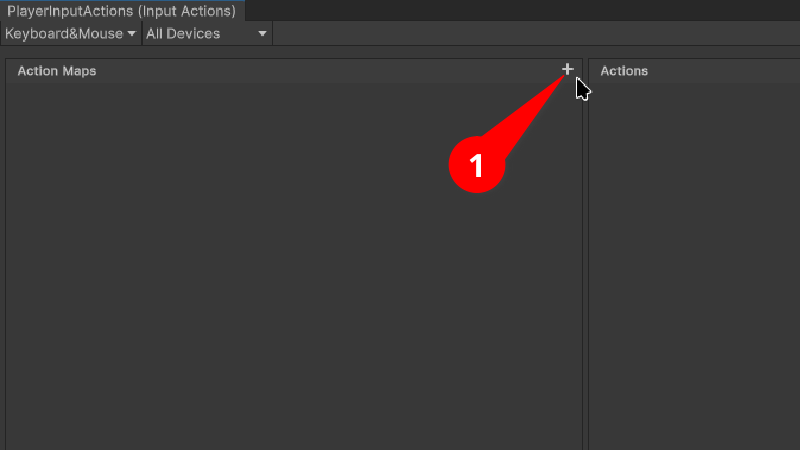
\includegraphics[width=.9\linewidth]{./SnapShots/AddMap.png}
\end{center}
We name our new \textbf{Action Map} as \emph{``Player''}.
\subsection*{Create New Binding}
\label{sec:org8faf7e8}
Unity creates an \textbf{Input Action} for us called \emph{``New action''//}. Rename this action \emph{``Jump''}. We'll set this action to be triggered by the space bar. We do this by creation a new \textbf{Binding}.
\begin{enumerate}
\item Under the \emph{``Jump''} action select \emph{``<No Binding>''}
\item In the \emph{``Binding''} panel select the drop down menu next to \emph{``Path''}
\item In the search bar search for space
\item Select \emph{``Space [Keyboard]''} in the search results
\begin{center}
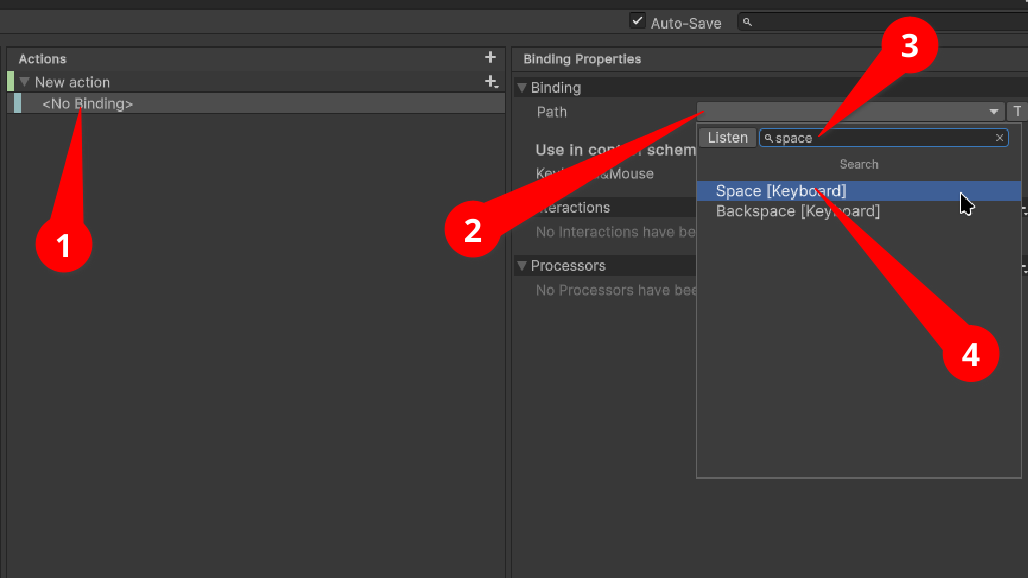
\includegraphics[width=.9\linewidth]{./SnapShots/AddBinding.png}
\end{center}
We repeat these steps but for a new \textbf{Input Action} called \emph{``Fire''//}. This time we search for \emph{``Left Button [Mouse]''} in the \emph{``Path''} drop down menu. Our Actions look like this after we are finished.
\begin{center}
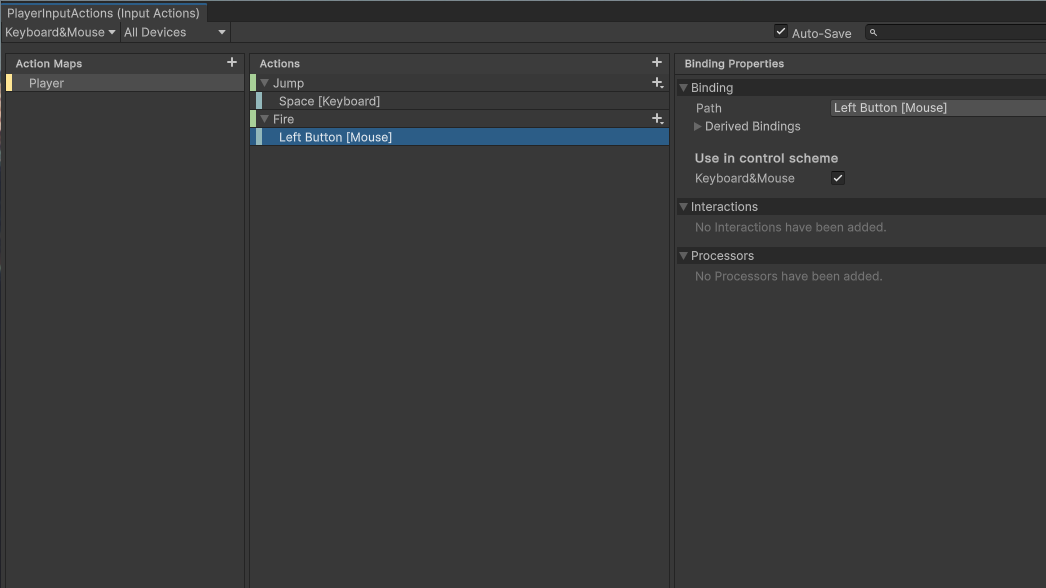
\includegraphics[width=.9\linewidth]{./SnapShots/FinalActions.png}
\end{center}
/newline
/newline
\end{enumerate}
Our \textbf{Input Actions} are now complete. Next we learn how to listen for when our events are triggered.
\section*{Using Input Actions}
\label{sec:org47288e1}
Every time the player presses their spacebar or clicks their left mouse button, our \emph{``Jump''} and \emph{``Fire''} \textbf{Input Actions} are triggered
\subsection*{Add Player Input}
\label{sec:org2cd097f}
We can listen for those events using the \textbf{Player Input} component. Create an empty game object in the project Hierarchy called \emph{``Player''//}. Add the \textbf{Player Input} component in the inspector for this \emph{``Player''} game object.
After adding the component:
\begin{enumerate}
\item In the \textbf{Player Input} component panel, select the \emph{``Actions''} radial button
\item Select your the \textbf{Input Action Asset} we created earlier
\item Select the \textbf{Control Scheme} we created earlier
\end{enumerate}
\begin{center}
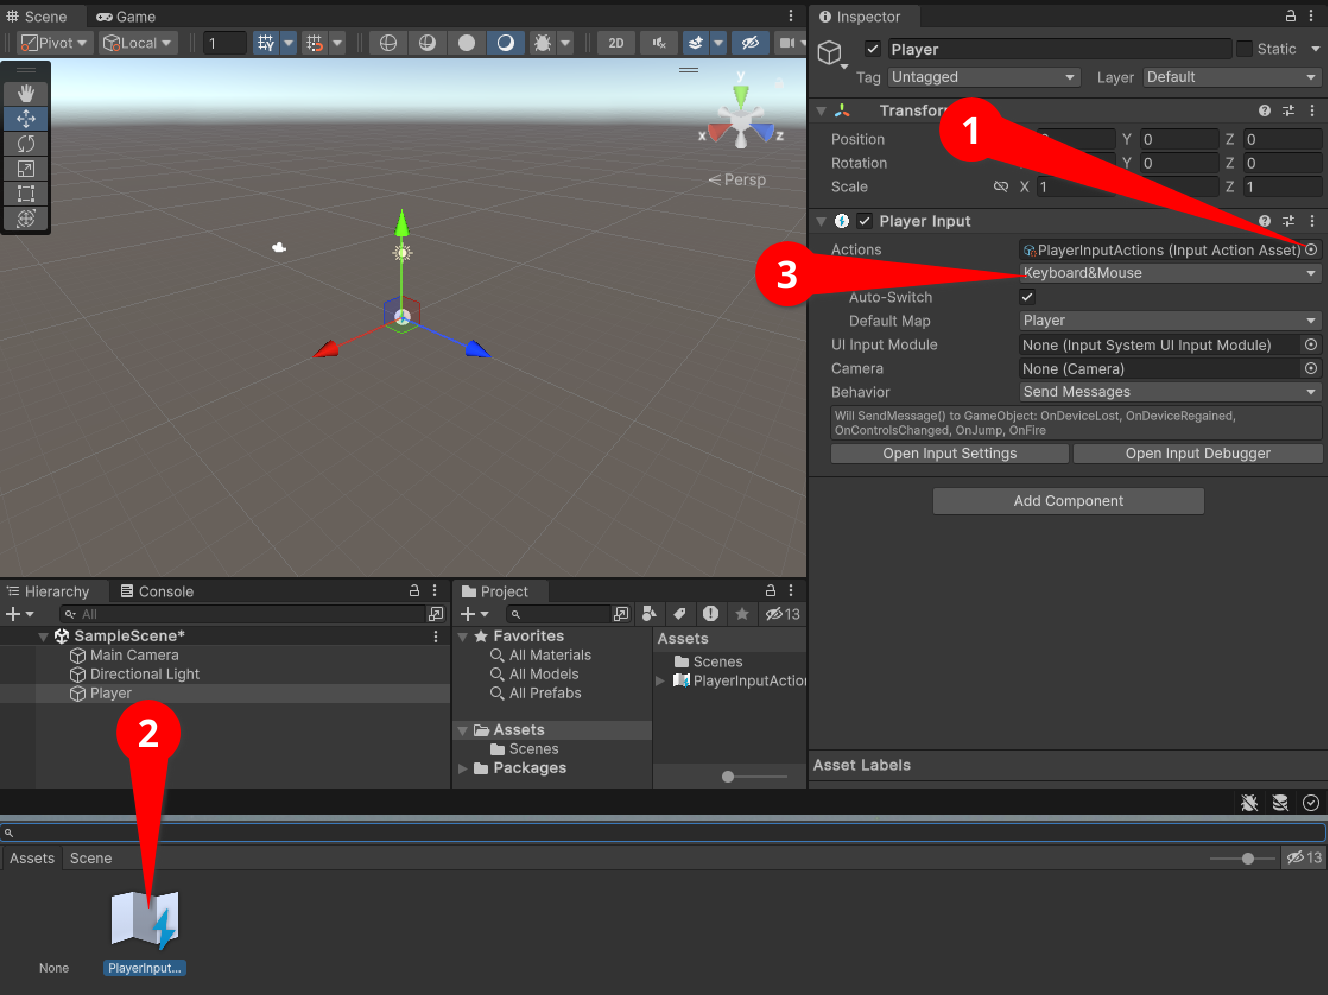
\includegraphics[width=.9\linewidth]{./SnapShots/AddPlayerInput.png}
\end{center}
Our player object is now linked to our \textbf{Input Actions}, \emph{``Jump''} and \emph{``Fire''}.
\subsection*{Add Logic to Input Action}
\label{sec:orgfc955dd}
Now that our player object is aware of our \textbf{Input Action} events we can add logic to them via a script. Add a new script to the \emph{``Player''} game object. In our example we name it \emph{``PlayerActions''}.
Add the following code snippet to the \emph{``PlayerActions.cs''} file.
\begin{verbatim}
using UnityEngine;

public class PlayerActions : MonoBehaviour
{
    // when the player creates the Jump event
    public void OnJump()
    {
        // print this message to the console
        Debug.Log("The Player created our Jump InputAction");
    }

    // when the player creates the Fire event
    public void OnFire()
    {
        // print this message to the console
        Debug.Log("The Player created our Fire InputAction");
    }
}
\end{verbatim}
With this code added to the player object, we've succeeded in writing custom logic that will come to define what our \textbf{Input Actions} do. Now when we play our game the message, \emph{``The Player created our Jump InputAction''//}, is printed when the player presses the spacebar. Or it will print \emph{``The Player created our Fire InputAction''}.
\section*{Why it Matters}
\label{sec:org6241bcb}
\href{https://gamedevbeginner.com/input-in-unity-made-easy-complete-guide-to-the-new-system/}{Input in Unity made easy} makes great points on why it is worthwhile to do this setup. Something it doesn't touch on however is how \textbf{Input Actions} promote good code. Creating the \emph{``PlayerAction.cs''} script demonstrates good compartmentalization of game logic. It pulls us away from putting all our logic into the \emph{``Update()''} method. It encourages an exciting design pattern that simplifies the difficult process of making a game.
\end{document}
